\documentclass{article}
\usepackage[UTF8]{ctex}
\usepackage{enumitem}
\usepackage{graphicx}

\begin{document}

\title{My Document}
\author{Smile Expression}
\date{\today}

\maketitle

\section{}

\subsection{}

概念:

把一张2D图片包裹3D物体,以模拟表面的细节和改观。

作用:

\begin{itemize}[leftmargin=2cm]
    \item 定义表面反射率的变化
    \item 描述表面材料特性
    \item 法线和置换贴图
    \item 计算的照明和阴影
    \item 添加细节
\end{itemize}

\subsection{}

只需两个简单的条件:

\begin{enumerate}[leftmargin=2cm]
    \item 每条“内部”边只包含在两个多边形中
    \item 每个“内部”点与顶点的连线构成一圈循环的多边形
\end{enumerate}

\subsection{}

\begin{tabular}{|c|c|c|c|}
    \hline
    原始颜色 & 原始RGB           & 实际RGB           & 实际颜色 \\
    \hline
    青色   & (0, 255, 255)   & (255,0,255)     & 洋红色  \\
    \hline
    洋红色  & (255, 0, 255)   & (0,255,255)     & 青色   \\
    \hline
    黄色   & (255, 255, 0)   & (255, 255, 0)   & 黄色   \\
    \hline
    黑色   & (0, 0, 0)       & (0, 0, 0)       & 黑色   \\
    \hline
    白色   & (255, 255, 255) & (255, 255, 255) & 白色   \\
    \hline
\end{tabular}

\section{}

\begin{figure}
    \centering
    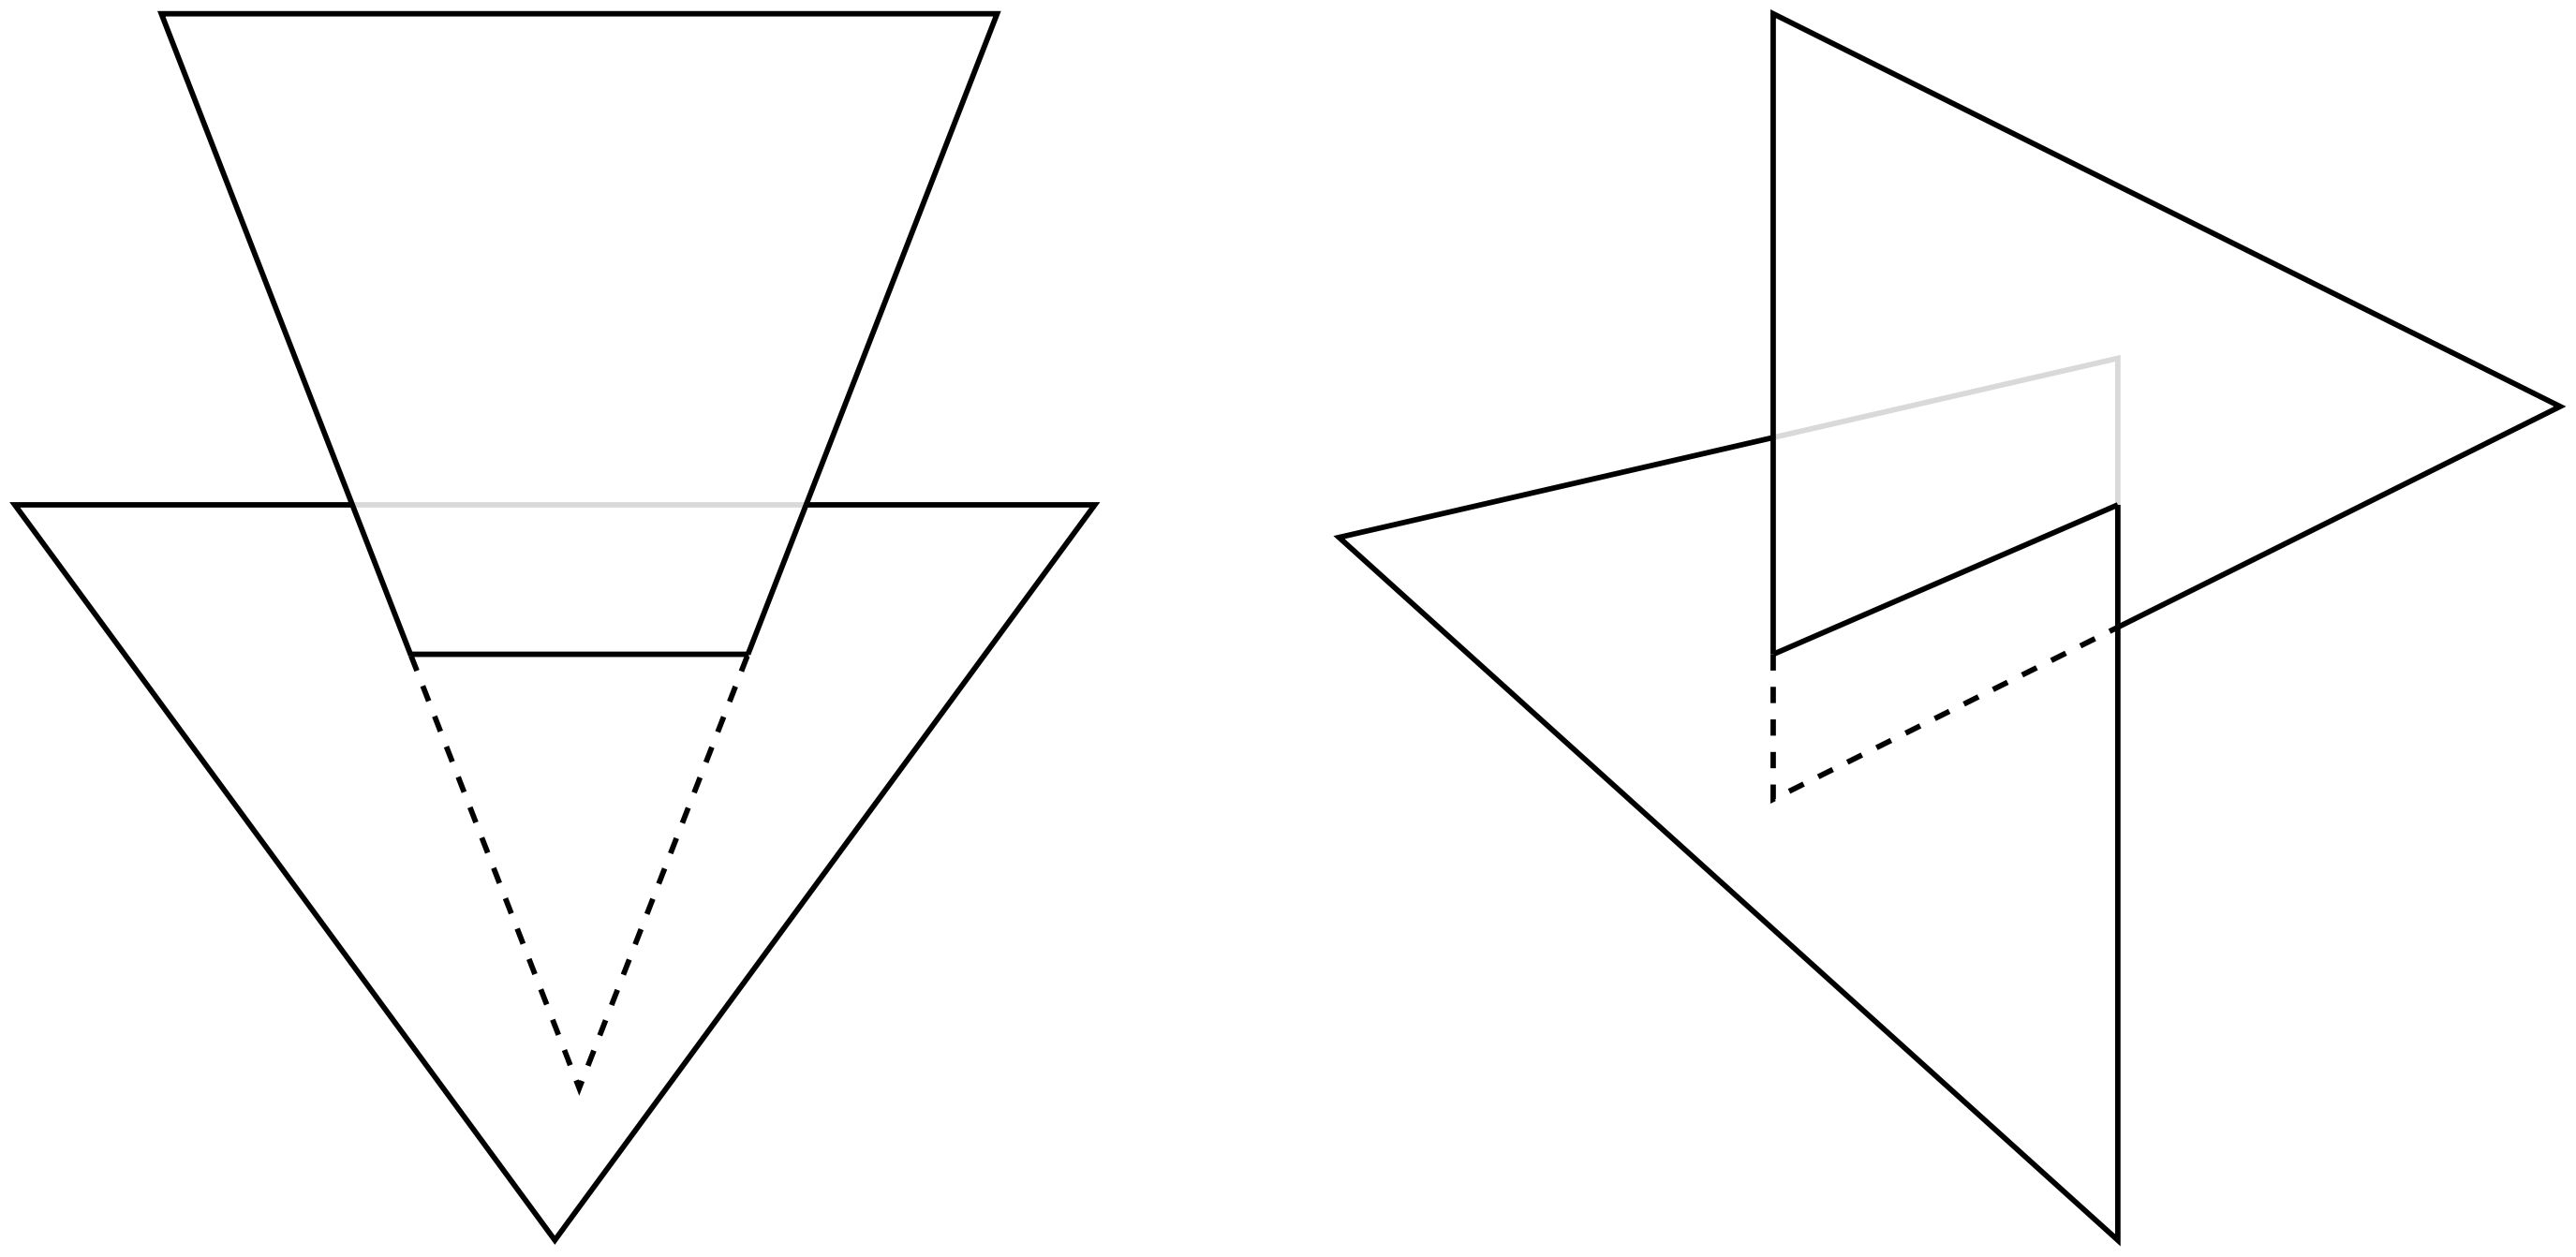
\includegraphics[width=0.8\textwidth]{pic/image-20231212174346327.png}
    \caption{两个三角形的相交情况}
    \label{fig:image}
\end{figure}

两个三角形相交:

\begin{itemize}[leftmargin=2cm]
    \item 要么一个三角形的两条边与另一个三角形相交(图1左侧)
    \item 或者两个三角形的一条边与另一个三角形相交(图1右侧)
\end{itemize}

步骤:检查第一个三角形的每一条边是否与第二个三角形相交,若有且仅有一条这样的边,说明两个三角形相交情况如图1右侧。若有两条边,说明相交情况如图1左侧。若没有这样的边,说明两个三角形不相交。

\end{document}
